% !TEX root = ./busty_transcription.tex
\section{Finding the ``right'' model: Bayesian parameter inference and model selection}
\subsection{Parameter inference for constitutive promoters}

From consideration of Fano factors in the previous section, we suspect that
model 5 in~\fig{fig:constit_cartoons}, a one-state bursty model of constitutive
promoters, achieves a Goldilocks level of complexity. Does this stand up to
closer scrutiny, namely, comparison to full mRNA distributions rather than
simply their moments? We will test this thoroughly on all the data from
constitutive promoters from Jones et.\ al.~\cite{Jones2014}.

It will be instructive, however, to first consider the Poisson promoter, model 1
in~\fig{fig:constit_cartoons}. This is a convenient proxy for models 2 and 3,
whose exact steady-state mRNA distributions would be tedious to calculate and we
will not explicitly consider. But since they have Fano factors $\nu\le 1$, they
can fare no better than the simple Poisson model. We will also not explicitly
consider model 4 from~\fig{fig:constit_cartoons} since it was already thoroughly
analyzed in~\cite{Razo-Mejia2020}, and since model 5 can be viewed as a special
case of it.

In performing parameter inference on the FISH data of~\cite{Jones2014}, building
a generative model is straightforward. The data are single-cell mRNA counts, and
we assume different cells to be independent and identically distributed from the
underlying generative model, which is just the steady-state mRNA distribution
computed from the master equation of the underlying model.

\subsubsection{Model 1: Poisson promoter}
\mmnote{A lot of the details I've written here might be excessive for main text and serve better as an intro-by-example to Bayes in the appendix, then reduce main text to a bit more bare bones?}
For this model the master equation of interest is~\eq{eq:poisson_promoter_cme}
with repressor set to zero, i.e.,
\begin{equation}
\deriv{t}p_{m,U}(t) = rp_{m-1,U}(t) - rp_{m,U}(t)
        + (m+1)\gamma p_{m+1,U}(t) - \gamma p_{m,U}(t),
\end{equation}
whose steady-state distribution is Poisson, given by
\begin{equation}
p_{m,U} = \frac{\lambda^m e^{-\lambda}}{m!}
\end{equation}
with $\lambda=r/\gamma$. This steady state distribution defines our likelihood
$p(m\mid\lambda)$, i.e.,
\begin{equation}
p(m\mid\lambda) = \frac{\lambda^m e^{-\lambda}}{m!}
\label{eq:poisson_inference010}
\end{equation}
is the probability of observing a single cell with $m$ mRNAs given a known value
of $\lambda$.

With our likelihood in hand, we can invoke Bayes theorem to write down the
posterior distribution on our model parameter $\lambda$, given by
\begin{equation}
p(\lambda\mid D) \propto p(D\mid\lambda) p(\lambda),
\end{equation}
where our data $D=\{m_1, m_2,\dots, m_N\}$ is a list of mRNA counts over a
population of $N$ identical cells. As is standard we have neglected the factor
$p(D)$ on the right hand side since it is independent of $\lambda$ and serves
only as a normalization factor. Since we assume each cell's mRNA count is
independent of others, the likelihood is simply a product of the single cell
likelihoods given by \eq{eq:poisson_inference010} above, so
\begin{equation}
p(D\mid\lambda) = \prod_{k=1}^N \frac{\lambda^{m_k}e^{-\lambda}}{m_k!}.
\end{equation}
This is often notated simply as
\begin{equation}
D\mid\lambda \sim \text{Poisson}(\lambda),
\end{equation}
which is read as the data $D$, conditioned on a value of $\lambda$, is Poisson
distributed with mean $\lambda$. The $\sim$ operator literally denotes ``is
distributed according to.''

To proceed we need to specify a prior. In this case we are extremely data-rich,
as the dataset from Jones et.\ al~\cite{Jones2014} has of order 1000-3000
single-cell measurements for each promoter, so our choice of prior matters
little here, as long as it does not exclude the true value of $\lambda$. A
convenient choice for our Poisson likelihood is its conjugate prior, the gamma
distribution. Although they only exist for certain special likelihoods,
conjugate priors have the nice feature that the posterior takes the same
functional form as the prior, with updated parameters. This makes calculations
analytically tractable and also offers a nice interpretation of the inference
procedure as updating our knowledge about the model parameters.

Putting a gamma prior on $\lambda$ introduces two new parameters $\alpha$ and
$\beta$ which parametrize the gamma distribution itself, which we use to encode
the range of $\lambda$ values we view as reasonable. Recall $\lambda$ is the
mean steady-state mRNA count per cell, which \textit{a priori} could plausibly
be anywhere from 0 to a few hundred. $\alpha=1$ and $\beta=1/50$ achieve this,
since the gamma distribution is strictly positive with mean $\alpha/\beta$ and
standard deviation $\sqrt{\alpha}/\beta$. To be explicit, then, our prior is
\begin{equation}
\lambda\mid\alpha,\beta \sim \text{Gamma}(\alpha, \beta)
\end{equation}

As an aside, note that if we did not know that our prior was a conjugate prior,
we could still write down our posterior distribution from its definition as
\begin{equation}
p(\lambda\mid D,\alpha,\beta)
\propto p(D\mid\lambda) p(\lambda \mid\alpha,\beta)
\propto \left(\prod_{k=1}^N \frac{\lambda^{m_k}e^{-\lambda}}{m_k!}\right)
        \frac{\beta}{\Gamma(\alpha)}(\beta\lambda)^{\alpha-1} e^{-\beta\lambda}
.
\end{equation}
Without foreknowledge that this in fact reduces to a gamma distribution, this
expression might appear rather inscrutable. When conjugate priors are
unavailable for the likelihood of interest - which is almost always the case for
models with $>1$ model parameter - this inscrutability is the norm, and making
sense of posteriors analytically is almost always impossible. Fortunately, MCMC
sampling provides us a powerful method of constructing posteriors numerically
which we will make use of extensively.

Since we did use a conjugate prior, we may simply look up our posterior in any
standard table of conjugate priors-likelihood pairs, from which we find that
\begin{equation}
\lambda\mid D,\alpha,\beta
\sim \text{Gamma}\left(\alpha + \bar{m}N, \beta + N\right),
\end{equation}
where we defined the sample mean $\bar{m} = \frac{1}{N}\sum_k m_k$ for
notational convenience. A glance at the FISH data from~\cite{Jones2014} reveals
that $N$ is $\mathcal{O}(10^3)$ and $\langle m\rangle \gtrsim 0.1$ for all
constitutive strains in~\cite{Jones2014}, so $\bar{m}N \gtrsim 10^2$. Therefore
as we suspected, our prior parameters are completely overwhelmed by the data. In
fact, $\bar{m}N$ and $N$ are so large that we can, to an excellent
approximation, ignore the $\alpha$ and $\beta$ dependence and approximate the
gamma distribution as a Gaussian with mean $\bar{m}$ and standard deviation
$\sqrt{\bar{m}/N}$, giving
\begin{equation}
\lambda\mid D
\sim \text{Gamma}\left(\alpha + \bar{m}N, \beta + N\right)
\approx \text{Normal}\left(\bar{m}, \sqrt{\frac{\bar{m}}{N}}\right).
\end{equation}
As an example with real numbers, for the \textit{lacUV5} promoter, Jones et.\
al~\cite{Jones2014} measured 2648 cells with an average mRNA count per cell of
$\bar{m} \approx 18.7$. In this case then, our posterior is
\begin{equation}
\lambda\mid D_{UV5}
\sim \text{Normal}\left(18.7, 0.08\right),
\end{equation}
which suggests we have inferred our model's one parameter to a precision of
order 1\%.

This is not wrong, but it is not the full story. The model's posterior is
tightly constrained, but is it a good generative model? In other words, does the
model generate data that look similar to our actual data, and is it therefore
plausible that the model captures the important features of the data generating
process? This intuitive notion can be codified with \textit{posterior predictive
checks}, or PPCs, and we will see that this simple Poisson model fails badly.

The intuitive idea of posterior predictive checks is simple: \mmnote{Not sure if
all this stuff is clearer by example, but then does it confuse the reader in
generalizing to other models?}
\begin{enumerate}
\item Make a random draw of the model parameter $\lambda$ from the posterior
distribution.
\item Plug that draw into the likelihood and generate a synthetic dataset
$\{m_k\}$ conditioned on $\lambda$.
\item Repeat many times.
\end{enumerate}
More formally, the posterior predictive distribution can be thought of as the
distribution of future yet-to-be-observed data, conditioned on the data we have
already observed. Clearly if those data appear quite different, the model has a
problem. Put another way, if we suppose the generative model is true, then the
synthetic datasets we generate should resemble the actual observed data, and if
not, it suggests the model is missing important features. All the data we
consider in this work are 1D (distributions of mRNA counts over a population) so
ECDFs are an excellent visual means of comparing synthetic and observed
datasets. In general for higher dimensional datasets, much of the challenge is
in merely designed good visualizations that can actually show if synthetic and
observed data are similar or not.

For our example Poisson promoter model then, we merely draw many random numbers,
say 1000, from the Gaussian posterior. For each one of those draws, we generate
a dataset from the likelihood, i.e., we draw 2648 (the number of observed cells
in the actual dataset) Poisson-distributed numbers for each of the 1000
posterior draws, for a total of 2648000 samples from the posterior predictive
distribution.

To compare so many samples with the actual observed data, one excellent
visualization for 1D data is ECDFs of the quantiles, as shown for our Poisson
model in~\fig{fig:uv5_post}. In this example, the median for each possible mRNA
count is shown as a dark green line, while shaded bands of progressively lighter
green contain 25\%, 50\%, 75\%, and 95\% of the posterior predictive samples.
Plotting quantiles in this way gives us a sense of the range of data we might
consider plausible, under the assumption that the model is true. In this case it
is quite obvious that the observed data, plotted in orange, could not plausibly
come from this Poisson generative model. The other model with a PPC plotted
in~\fig{fig:uv5_post}, bursty model 5 with a negative binomial steady-state mRNA
distribution, looks like a good candidate by eye. We cover it in more detail
later.

\begin{figure}%[h!]
\centering
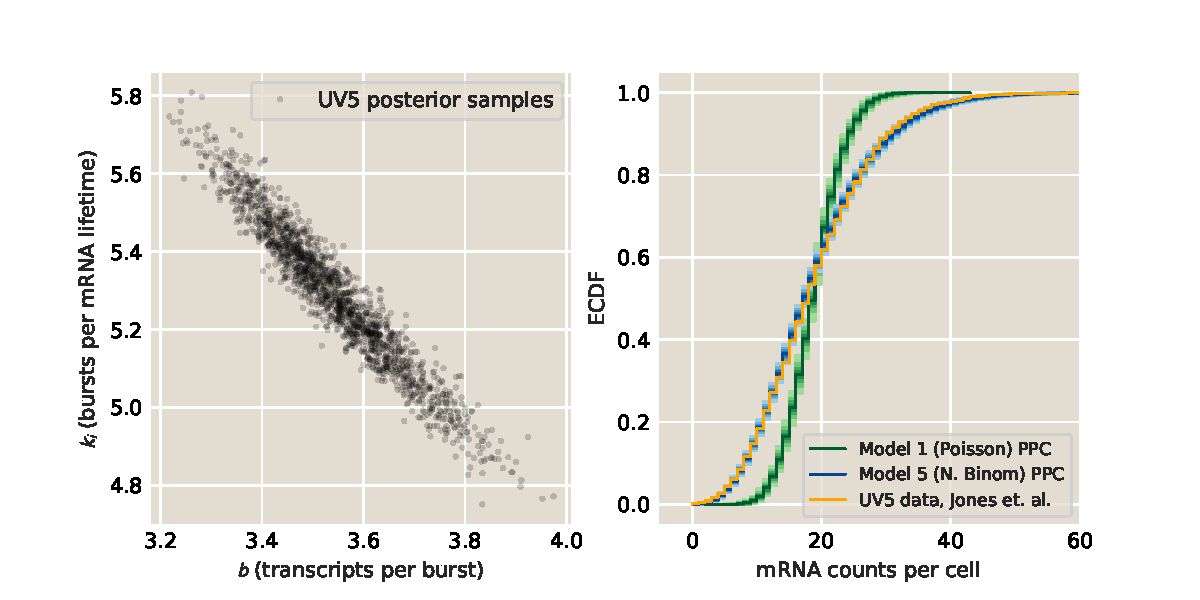
\includegraphics[width=0.9\textwidth]{../figures/fig2/fig2pt1.pdf}
\caption{\textbf{Constitutive promoter posterior inference and predictive
        checks.} (A) shows the joint posterior density from MCMC sampling of
        model 5, bursty promoter with negative binomially-distributed steady
        state. (B) shows the ECDF of the observed population distribution of
        mRNA transcripts under the control of a constitutive lacUV5 promoter.
        Posterior predictive percentiles are shown as colored bands for model
        (1), Poisson, and model (5), negative binomial.}
\label{fig:uv5_post}
\end{figure}
        
\mmnote{Outline, still to cover:
\begin{itemize}
\item Bursty model. Write Bayes, sketch story of NB likelihood, sketch choice of
priors, show~\fig{fig:uv5_post}, see bursty $\gg$ Poisson model.
\item All 18 promoters. Hey the model still works on things other than UV5,
cool. Interesting and somewhat counterintuitive scaling b/w burst rate and
binding energy. Puzzle in comparing w/ Chong2014 supercoiling model. Are we
missing important things?? Unclear, we leave as open question. Good enough for
our purposes: posterior is identifiable, PPC is great, and of the models we've
thought of it is unique in satisfying both.
\end{itemize}
}

\begin{figure}%[h!]
\centering
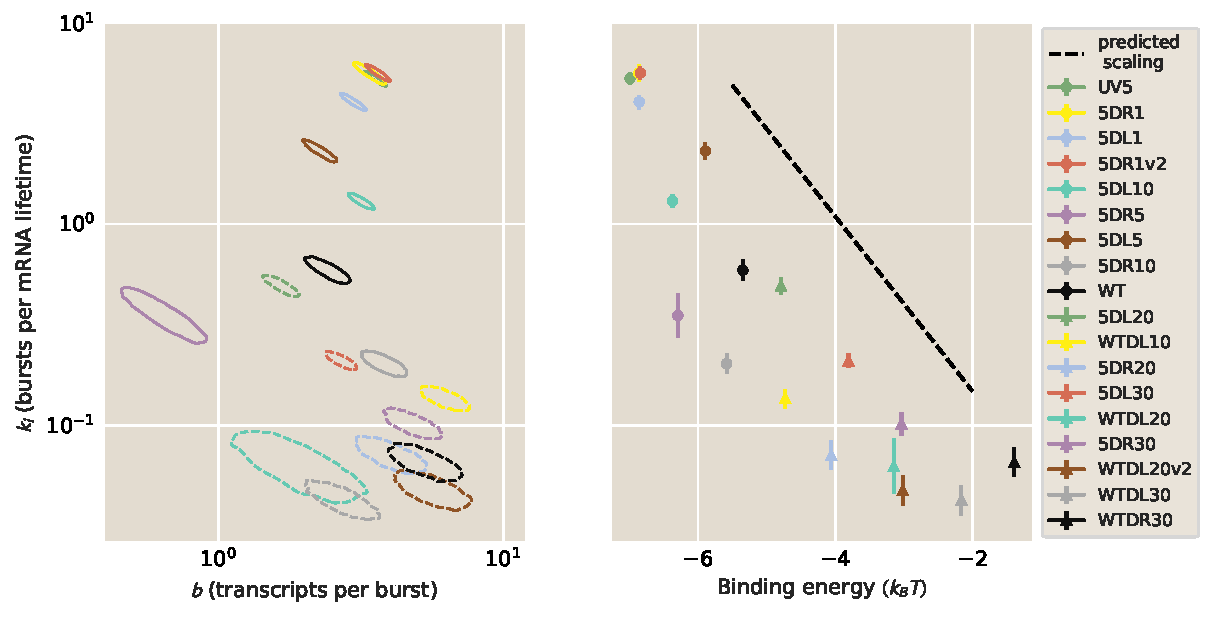
\includegraphics[width=0.9\textwidth]{../figures/fig2/fig2pt2.pdf}
\caption{\textbf{Constitutive promoter model comparison.}
    (A) Joint posterior distributions for burst rate $k_i$ and mean burst size
    $b$ for 18 promoters from Jones 2014. Each contour indicates the 95\%
    highest posterior density region for a particular promoter, i.e., on a plot
    analogous to~\fig{fig:uv5_post}, the contour would enclose approximately
    95\% of the samples, and thus 95\% of the probability mass. Note that the
    vertical axis is shared with (B). Panel (B) plots the burst rate $k_i$ vs.\
    binding energy from energy matrices from Brewster 2012. The dotted line
    shows the predicted slope according to $\ln k_i/\gamma \sim \text{constant}
    - \beta\Delta\epsilon_P$, described in text.}
\label{fig:constit_post}
\end{figure}
\mmnote{Discuss puzzling comparison w/ Chong2014: if supercoiling is the thing, why are my burst sizes all the same but burst rates vary? And why is the duty cycle of my promoter so low, ie., bursts so short? COmpare their fig 7E; their $\beta/\alpha$ is my $k^+/k^-$. They have one or two genes with very small $\beta/\alpha$, does the \textit{galK} locus just happen to be that, or is there a deeper disagreement? Hard to say w/o more data.}

\subsection{Transcription factor kinetics can be inferred from FISH measurements}
\mmnote{Outline:
\begin{itemize}
\item Full model. Write Bayes, handwave 2F1 dist story in limits of weak,
strong, and intermediate repression.
\item Hey look it mostly works. With full model, 9D model is well identified,
though most of the individual experiments unsurprisingly are not: only the ratio
of repressor rates is identifiable. PPC is not perfect, it kinda misses some
rep/op pairs but overall it's surprisingly predictive considering how strong
were the assumptions that went into it.
\item Do we chalk this up to experimental imperfections or is there interesting
biology to be found in the disagreements? I'm inclined towards the former. Even
just catching cells in truly apples-to-apples growth phases, or matching up
parameters of imaging sessions weeks or months apart, is hardly trivial.
\item The alternative is to refine our model and/or add on complexity, and it's
not at all clear what additions to make to the model, especially how to produce
the long tail of repressed strains over UV5. I see no way to get that without
getting into complicated time-correlation/history effects, where
transcription...rebounds?? After being repressed?? Sounds odd.
\item Comparison between my inferred rates, equilibrium binding E, and
single-molecule measurements. Not quite as slam-dunk as I'd hoped because of
$\gamma$ dependence, but rates are w/in factor of 2 or better, seems quite good
really! With exception of one Oid data data point, free energies are w/in about
0.5 kT also. That's not massively larger than the repeatability threshold of
fold-change measurements, at maybe 0.1 to 0.3 kT.
\item Surprising that so many model parameters can be inferred from just a few
distributions that, by eye, don't have strong features! Does require some
assumptions, e.g., about equivalence of rates across experiments, but that seems
quite reasonable.
\end{itemize}
}

Figure~3 presents inferred transcription factor rates, compares them to
single-molecule measurements, and compares their ratios to gold-standard binding
energies.
\begin{figure}%[h!]
\centering
\includegraphics[width=0.9\textwidth]{../figures/fig3/fig3.ai}
\caption{\textbf{Simple repression model comparison.}
(A) depicts the cartoon of simple repression for which we infer parameters.
\mmnote{Not sure panel (A) is necessary, we've already shown it in at least 2
other figs. We could instead show some alternative slices of 9D posterior as a
companion to (B), or something totally different\dots??} (B) shows 50\% and 95\%
contours of several 2D slices of the 9D posterior distribution, from fitting one
unbinding rate for each operator (O1, O2, O3) and one binding rate for each aTc
concentration (corresponding to an unknown mean repressor copy number). (C)
compares ratios of our inferred unbinding rates with operator binding energy
differences measured in Garcia \& Phillips 2011 (triangles) and Razo-Mejia et.\
al.\ 2018 (squares). (D) compares our inferred unbinding rates with
single-molecule measurements of the same from Hammar et.\ at.\ 2014
\mmnote{Johan Elf's group}. Values are of similar order of magnitude, but a
precise quantitative comparison unfortunately depends sensitively on the assumed
mRNA lifetime, which was not measured.}
\label{fig3:kR_inferences}
\end{figure}

\begin{figure}%[h!]
\centering
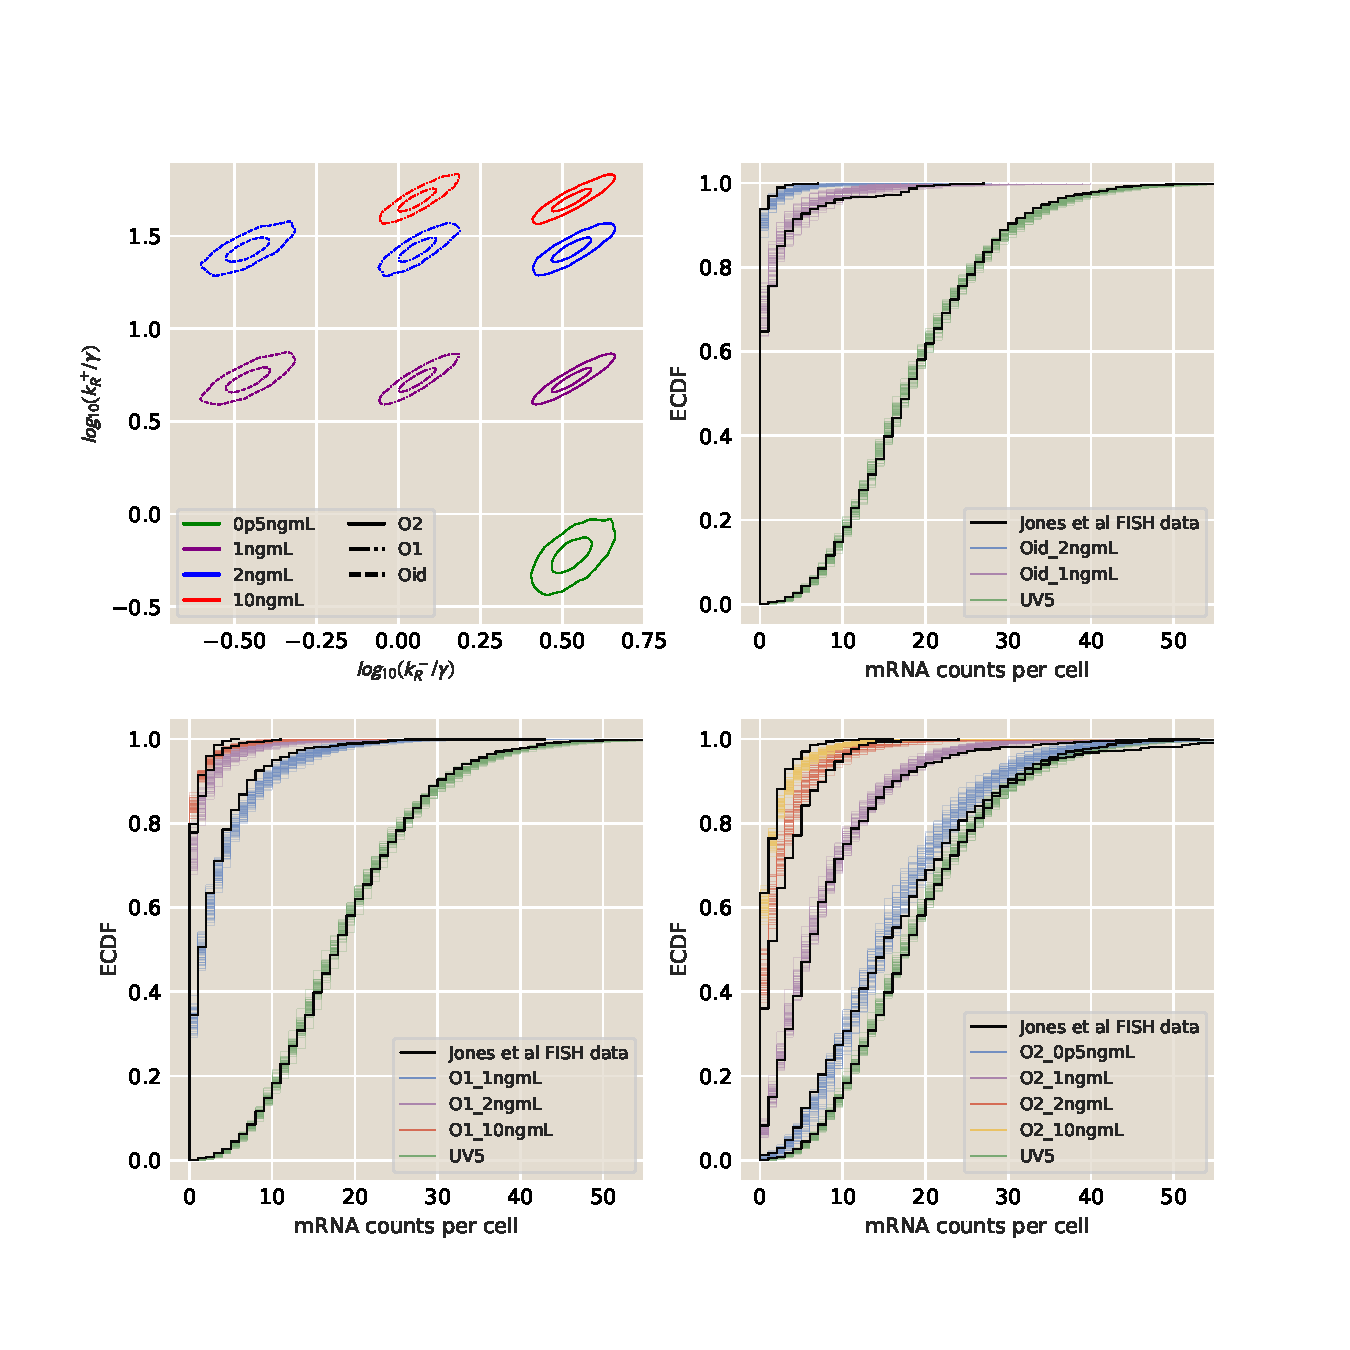
\includegraphics[width=0.9\textwidth]{../figures/figSIxx/ppc_many_pooled.pdf}
\caption{\textbf{Posterior predictive checks.}
(A) duplicates the posterior from~\fig{fig3:kR_inferences}B. (B), (C), and (D)
show samples from the posterior predictive distribution for each of the datasets
used in the inference. Samples are sorted by operator and plotted separately
simply for visual clarity. The unrepressed promoter, UV5, is shown with each as
a reference point. \mmnote{Obviously the PPC is not perfect, but considering the
relative simplicity of the model, I'm pleasantly surprised how well it worked
and that the model was even identifiable at all. Interestingly, and perhaps not
surprisingly, only 3 of the 9 datasets were identifiable if fit in isolation:
otherwise, it was only by making assumptions that certain rates are equal across
datasets was identifiability achieved.}}
\label{fig4:ppc}
\end{figure}